\section{Organisation of the team}
\label{sec:organization}

\subsection{Planning}

The work followed the two phases of the subject. The first one, until the analysis report,
covered the exploration of the NASA API, the specifications and the design. The second one
covered the implementation, with the database first, since every other component depends on it,
then the required features, the optional ones and the Streamlit interface. Figures
\ref{fig:gantt1} and \ref{fig:gantt2} show the planning made in the analysis report.

\begin{figure}[H]
  \centering
  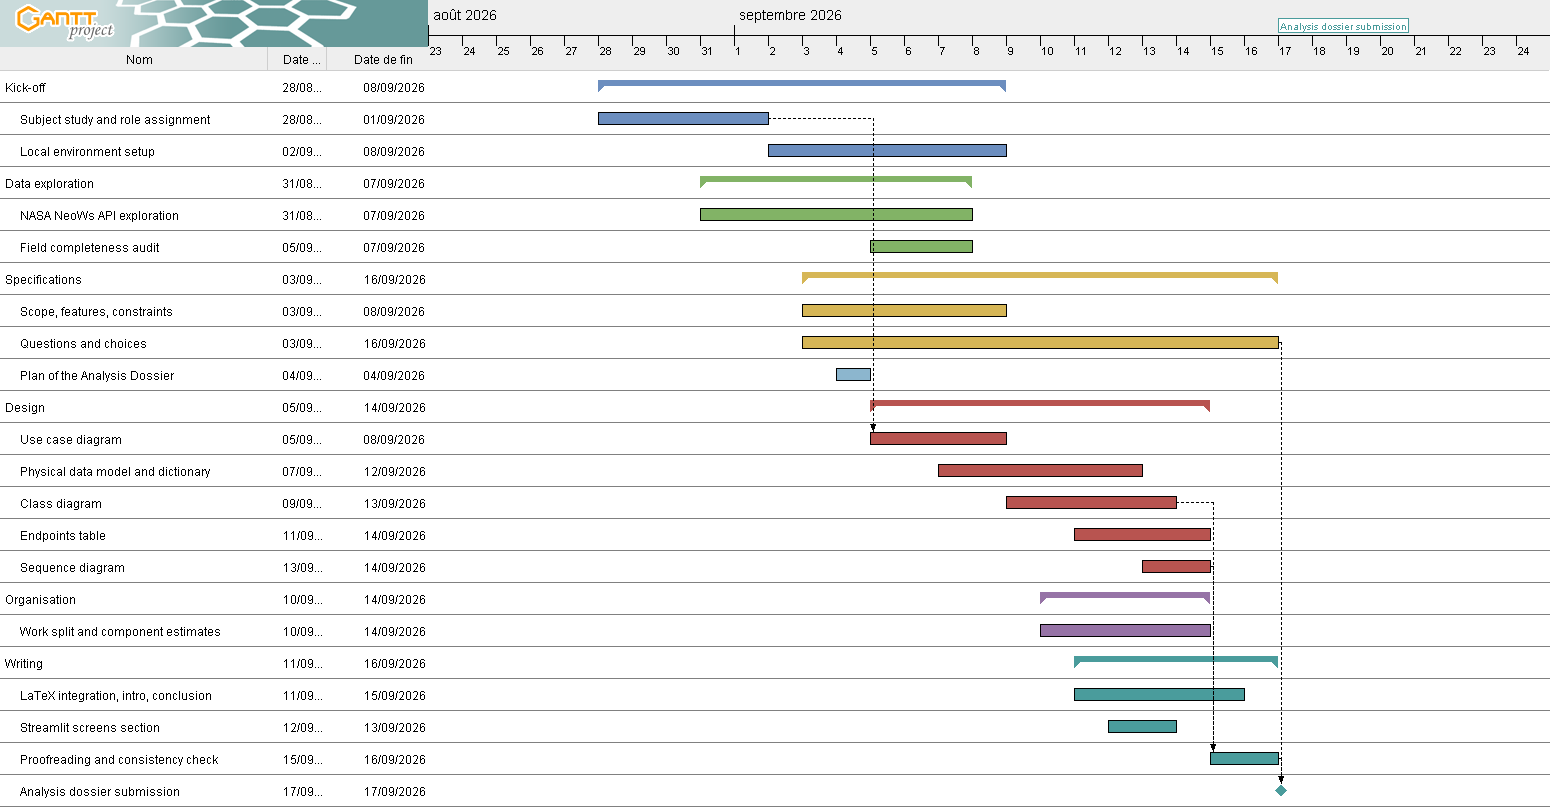
\includegraphics[width=0.8\textwidth]{NEO-Watch_gantt_phase1.png}
  \caption{Planned Gantt chart, phase 1}
  \label{fig:gantt1}
\end{figure}

\begin{figure}[H]
  \centering
  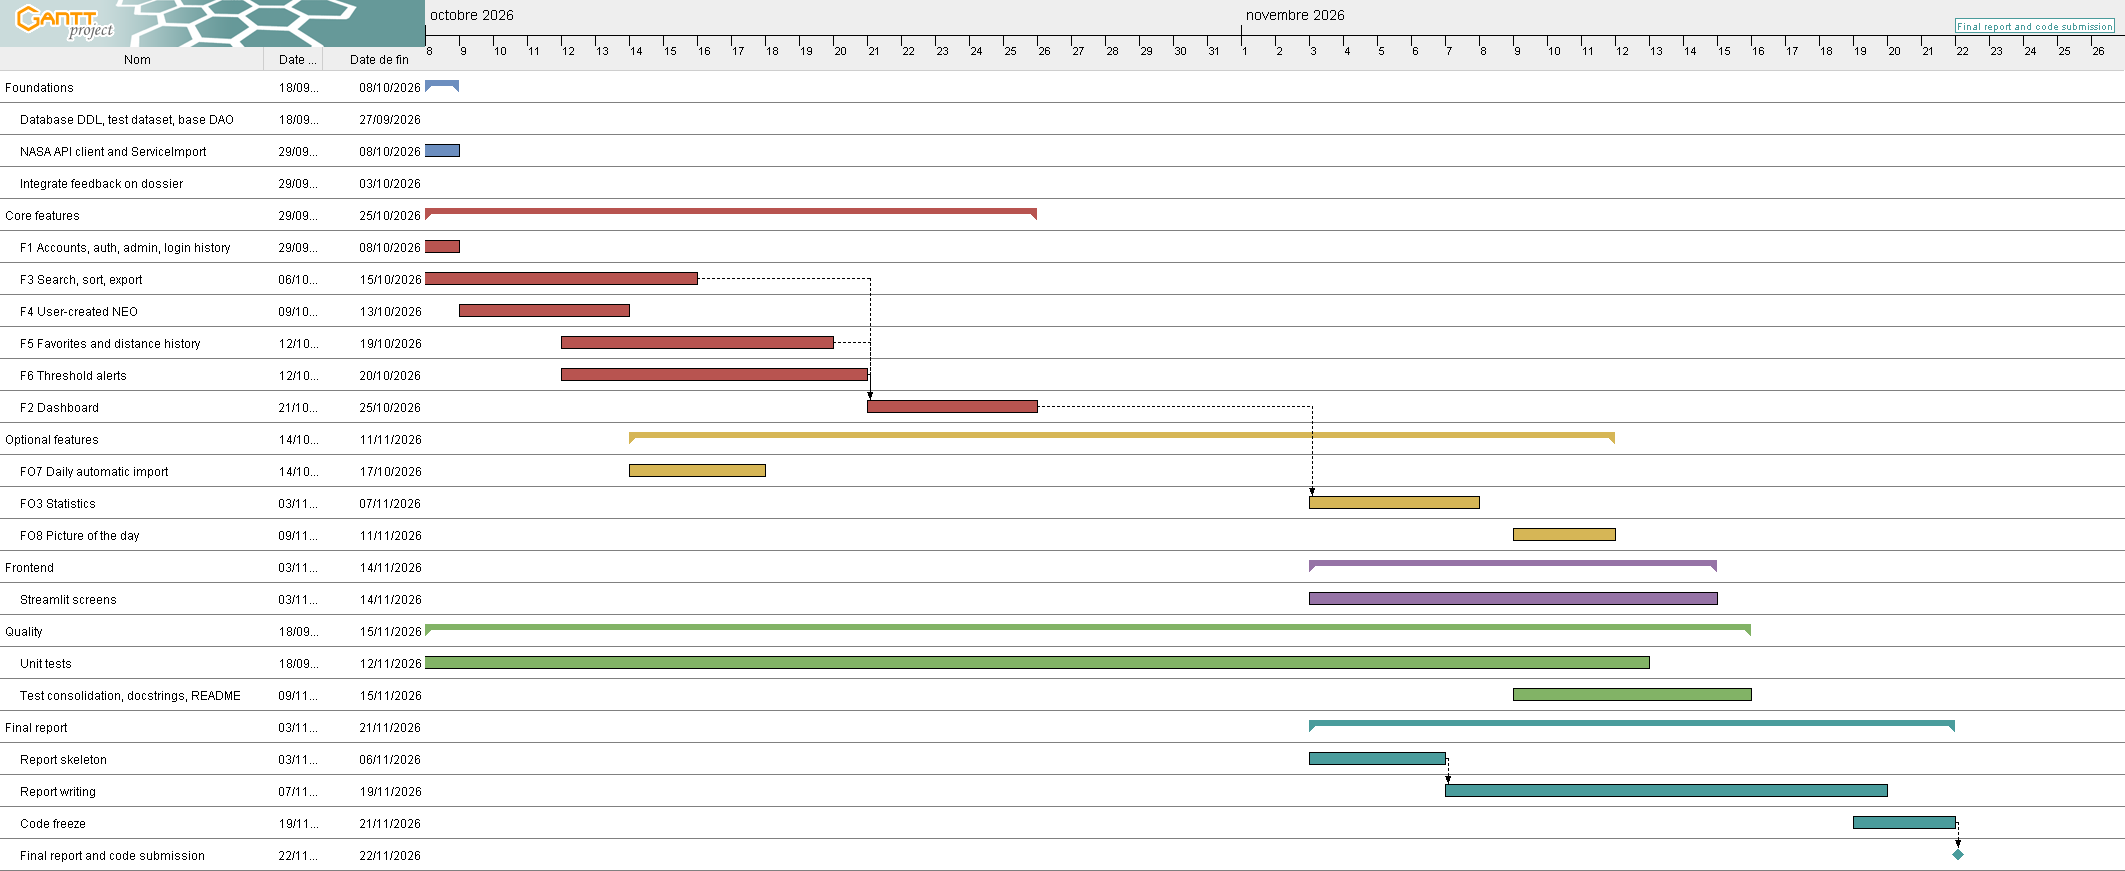
\includegraphics[width=0.8\textwidth]{NEO-Watch_gantt_phase2.png}
  \caption{Planned Gantt chart, phase 2}
  \label{fig:gantt2}
\end{figure}

In practice, the backend layers were built feature by feature rather than layer by layer, and
the integration of the whole application (running the API and the interface together) started
later than planned, in week 10. Several problems only appeared at that time: startup errors of the
backend, inconsistent return types between the controllers and the pages, and the database reset.
The last weeks were therefore devoted to integration, security, tests and documentation.

\subsection{Distribution of the work}

Each member was in charge of features from the database to the interface, which limited the
dependencies between members. Table~\ref{tab:roles} gives the main contributions, as recorded in
the weekly tracking documents (\texttt{doc/tracking/}).

\begin{table}[H]
\centering
\small
\begin{tabularx}{\textwidth}{l X}
\toprule
\textbf{Member} & \textbf{Main contributions} \\
\midrule
Sofia Bounaga & F1: \texttt{UserDao}, \texttt{ConnectionDao}, \texttt{UserService} and its tests; start of the JWT authentication; conventions shared between the layers \\
Yalalt Schneider & F5 and F6: favourites and alerts (DAO, services, controllers, pages) and their tests; integration of the NASA import in the interface \\
Valentin Denni & Business objects, NEO DAO, F3 and F4; backend startup and integration; JWT checks on the endpoints; tests, continuous integration and documentation; resumable import \\
Mohammed-adam Lakhrissi & F2 dashboard, FO3 statistics and FO8 picture of the day (from the DAO to the page) and their tests; tests of the installation from scratch \\
\bottomrule
\end{tabularx}
\caption{Main contributions of each member}
\label{tab:roles}
\end{table}

\subsection{Tools and methods}

\begin{itemize}
  \item \textbf{Git and GitHub}: one shared repository; features developed on branches and merged
  through pull requests or directly on \texttt{main}; about 200 commits.
  \item \textbf{Weekly follow-up}: a tracking document per week lists the tasks done by each
  member and the backlog, and is reviewed at the meeting with our advisor.
  \item \textbf{Shared conventions}: the vocabulary fixed in the analysis report (``NEO'',
  ``approach'', ``favourite'') is used in the class diagram, the tables, the classes and the
  endpoints.
  \item \textbf{Development environment}: SSP Cloud services (VSCode and PostgreSQL), with the
  configuration in a \texttt{.env} file that is not versioned.
\end{itemize}
